\section{Introduction} \label{sec:intro}
Monitoring and modeling of large-scale stochastic phenomena with both spatial and temporal (spatiotemporal) evolution using a network of distributed sensors is a critical problem in many controls applications. Consider, for example, a team of robots with the task of destroying herbicide-resistant weeds on a farm (see Figure \ref{fig:cps}, also see ``\nameref{sb:ag}''). This team of robots needs to predict weed growth across the whole farm  to make intelligent, coordinated decisions \cite{McAllistar18IROS}. However, the robots can only observe a limited part of the field at a time, leading to the critical problem: How can a few robots which can only partially observe the field at any time predict the full state of the spatiotemporally-evolving weed growth over the entire field? When building an observer over a spatiotemporal process, which locations should be sampled to obtain the necessary information to render the problem observable? The goal of this tutorial is to show the steps we have taken towards addressing this kind of challenging problem. Examples of such problems abound across many domains, including: modeling and monitoring of ocean heat content and acidification for oceanography using a network of satellites and surface sensors \cite{barnett2001detection}; prediction of traffic patterns using data from vehicles, cellphones, and traffic cameras; prediction of enemy movements through ground and aerial surveillance; and prediction of extreme weather events using data from weather stations and aerial drones \cite{heaton2011spatio}. The rapid advances in the computational power of compact systems and robotics as a whole has led to an explosion of real-world applications for such distributed cyber-physical systems. 
 
\begin{figure}[h] %{r}{0.5\textwidth}
	\centering
	\includegraphics[width=\columnwidth]{"Figure 1"}
		\caption{A Cyber Physical system consisting of a distributed team of robots for mechanical weed management on a farm. Image courtesy EarthSense inc.}
	\label{fig:cps}
\end{figure}


These types of applications need to estimate complex, stochastic dynamics that are distributed over space and time. The key constraint is the number of spatially distributed sensors available, which are not enough to entirely cover the whole space at any given moment in time. One approach to solving the problem under this constraint is to use a predictive model of the phenomenon which informs our sensing strategy. %It may be difficult to model such systems with spatiotemporal dynamics using first principles alone. 
While the modeling of such spatiotemporal phenomena has traditionally been the object of study in geostatistics, it has in recent years gained more attention in the machine learning community \cite{cressie2011statistics}. The data-driven models developed by machine learning techniques provide a way to capture complex spatiotemporal phenomena which are not easily modeled by first-principles alone. However, these models are limited by the data sets they are trained on, and the high variability of complex distributed physical systems makes it even more challenging. For example, a model trained over years of weed growth data in one field doesn't necessarily generalize to another, and a model trained on the past few years of data still cannot reliably predict weather variability in the following year. What is needed is not just a \textit{predict} system but a \textit{predict-and-correct} system. This tutorial shows how to design just such a system for these kind of problems. The system utilizes kernel methods for modeling, Bayesian filtering theory for prediction correction, and exploits the mathematical structure of the regression and dynamics models to place the sensors. 


In the machine learning community, kernel methods represent a class of well-studied and powerful methods for regression in spatial domains. In these techniques, correlations between the input variables are related via covariance kernels, and the model is generated by a linear combination of the kernels \cite{RasmussenWilliams2005,schoelkopf01kernelbased,scholkopf2002learning}. In recent years, kernel methods have been applied to spatiotemporal regression problems with varying degrees of success \cite{cressie2011statistics,RasmussenWilliams2005}. Many recent methods have focused on nonstationary covariance kernel design and algorithms for learning the associated hyperparameters \cite{garg2012AAAI,ma2003nonstationary,plagemann2008nonstationary,todescato2017efficient}. These methods, which focus on the careful design of covariance kernels, have been proposed as an alternative to the naive approach of simply including time as an additional input dimension in the kernel \cite{Chowdhary13_CDC1}. The careful design/optimization of a covariance kernel avoids an explosion in the number of parameters used by the model, which would be inevitable in the naive approach, and can better account for spatiotemporal couplings. Such covariance kernels, however, do not scale in the face of large-scale phenomena since the optimization of the kernel hyperparameters is non-convex and computationally demanding for large datasets \cite{sra2012optimization}. Deep learning also suffers from similar issues, and moreover lacks the spatial encoding properties of certain kernels, which are exploited by the strategy outlined in this tutorial.

No matter how much data the model is trained on, it cannot completely capture the variability of real-world systems with complex spatiotemporal dynamics. This is a problem that the controls community is quite aware of; their solution to this is built upon feedback, leading to fundamental notions of observability and controllability which can be used to build robust state estimators and controllers. To bring these ideas to fruition in the spatiotemporal problem, we needed a way to find where sensing/control should be performed to ensure that the state estimation problem can be made observable/controllable. % Current ML models do not provide such insight. In particular, 
%\rr{
While methods such as \cite{todescato2017efficient} have succeeded in using nonstationary kernels that evolve efficiently using feedback, it is not clear how notions of observability and controllability could be utilized with it or other existing kernel-based machine learning models, and how observers and controllers can be embedded within such models.
%} % for the large scale spatiotemporal phenoemena. }
Computational challenges can be addressed with faster methods or increasing computational power; however, addressing the latter, more fundamental challenge in designing robust observers/controllers is particularly important in the design of reliable engineering systems, such as distributed sensor/actuator networks intended for monitoring physical phenomena, autonomous soft-robots, or other physical systems with distributed sensing and actuation.



\subsection{Contributions}
In this tutorial, we present a different perspective on solving the spatiotemporal monitoring problem that brings together kernel-based modeling, systems theory, and Bayesian filtering. We define the monitoring problem as follows: \textit{given an approximate predictive model of the spatiotemporal phenomena learned using historical data, estimate the current latent state of the phenomena in the presence of uncertainty, using as few sensors as possible}. Ideally, the solution to the problem should also provide guidance on how many sensors are needed and where to place them. In this paper we argue that when it comes to predictive inference over spatiotemporal phenomena, a Kalman-filter type approach of predicting and correcting with feedback from a set of minimal sensors is a robust way of dealing with real-world uncertainties and inherent modeling errors.  In the context of this specific problem, our main contributions are two-fold: first, we demonstrate that spatiotemporal functional evolution can be modeled using stationary kernels with a linear dynamical systems layer on their mixing weights. In particular, in contrast with existing work, this approach does not necessarily require the design of complex spatiotemporal kernels, and can accommodate positive-definite kernels on any domain on which it is possible to define them, which includes non-Euclidean domains such as Riemannian manifolds, strings, graphs and images \cite{Jayasumana_PAMI2015_RBFs}. Second, we show that such a model can be utilized to determine sensing locations that guarantee that the hidden states of functional evolution can be estimated using a Bayesian state-estimator (Kalman filter) that is embedded in the feature space of the kernel model with very few sensors. A benefit of our solution's approach is that it provides guidance on how many sensors are needed and where to place them. Accordingly, we provide sufficient conditions on the number and location of sensor measurements required and prove non-conservative lower bounds on the minimum number of sampling locations by developing fundamental results on the observability of kernel-based models. Our model is also analyzed in terms of Koopman operator theory, and several key theoretical results are proven showing that our model can produce the Koopman modes, eigenvalues, and eigenfunctions. 
The validity of the presented model and sensing techniques is corroborated using synthetic and large real datasets. 

\subsubsection*{Broader Context}
The fundamental idea of building observers and controllers embedded in the feature spaces of machine learning models introduced in this paper is generalizable beyond the particular application of spatiotemporal monitoring. Figure \ref{fig:cps_soa} shows a general landscape of problems that are relevant for engineering. Since the controls literature is strongest when the system dynamics can be represented as Ordinary Differential Equations (ODEs), some of the major successes of controls have included results such as Linear Quadratic Gaussian control, reinforcement learning, and adaptive control in state spaces with well-defined, finite, and \emph{physically meaningful} state variables. The estimation of the states of these temporally evolving, finite-dimensional state-space systems have been extensively studied in the context of Kalman filtering and observer design \cite{Gelb74}. A different approach for modeling complex spatiotemporal dynamical systems comes from machine learning, where trained models reside in abstract feature spaces that are only relatable to physical quantities through complex functional operations (see ``\nameref{sb:featspace}''). There has been some work that relates approaches from controls to machine learning (see e.g. \cite{mardia1998kriged} for an extension of the Kalman filter to the functional domain), but the results are not studied in the context of the spatiotemporal monitoring problem presented here. 

To fuse machine learning with controls for building robust systems for engineering, we need to answer fundamental questions such as 1) the least number of sensors required to observe a distributed system, 2) the placement of sensors/actuators to guarantee observability/controllability of the system, and 3) the effect of random sensor placement on system observability/controllability.

This tutorial presents an approach that can provide one formal way of addressing these and other questions about complex systems that are modeled with machine learning. In particular, we demonstrate how linear dynamical systems can be embedded in the reproducing kernel Hilbert space (RKHS) \cite{schoelkopf01kernelbased,ams:cucker,kingravi2012reproducing} generated by features used in Gaussian Process modeling \cite{Liu2018csmtutorial,rasmussen2006gaussian}, %machine learning feature spaces 
and utilized to answer fundamental questions such as controllability and observability. 
% The marriage of systems theory with machine learning pursued in this paper is exciting, and % because it can provide a formal way of answering fundamental questions about complex systems, such as: % and seek to develop machine learning models that can be utilized to answer questions such as: 
We expect that follow-up work will exploit the framework presented in this paper of utilizing linear models in RKHSs and feature spaces of other machine learning models to enable practical and analyzable data-driven engineering systems. To facilitate the development of the theory, we have focused this paper on the problem of monitoring spatiotemporal phenomena. However, the idea should be generalizable to any distributed cyber-physical system that is changing with space and time. 

\begin{figure}[h] %{r}{0.5\textwidth}
	\centering
	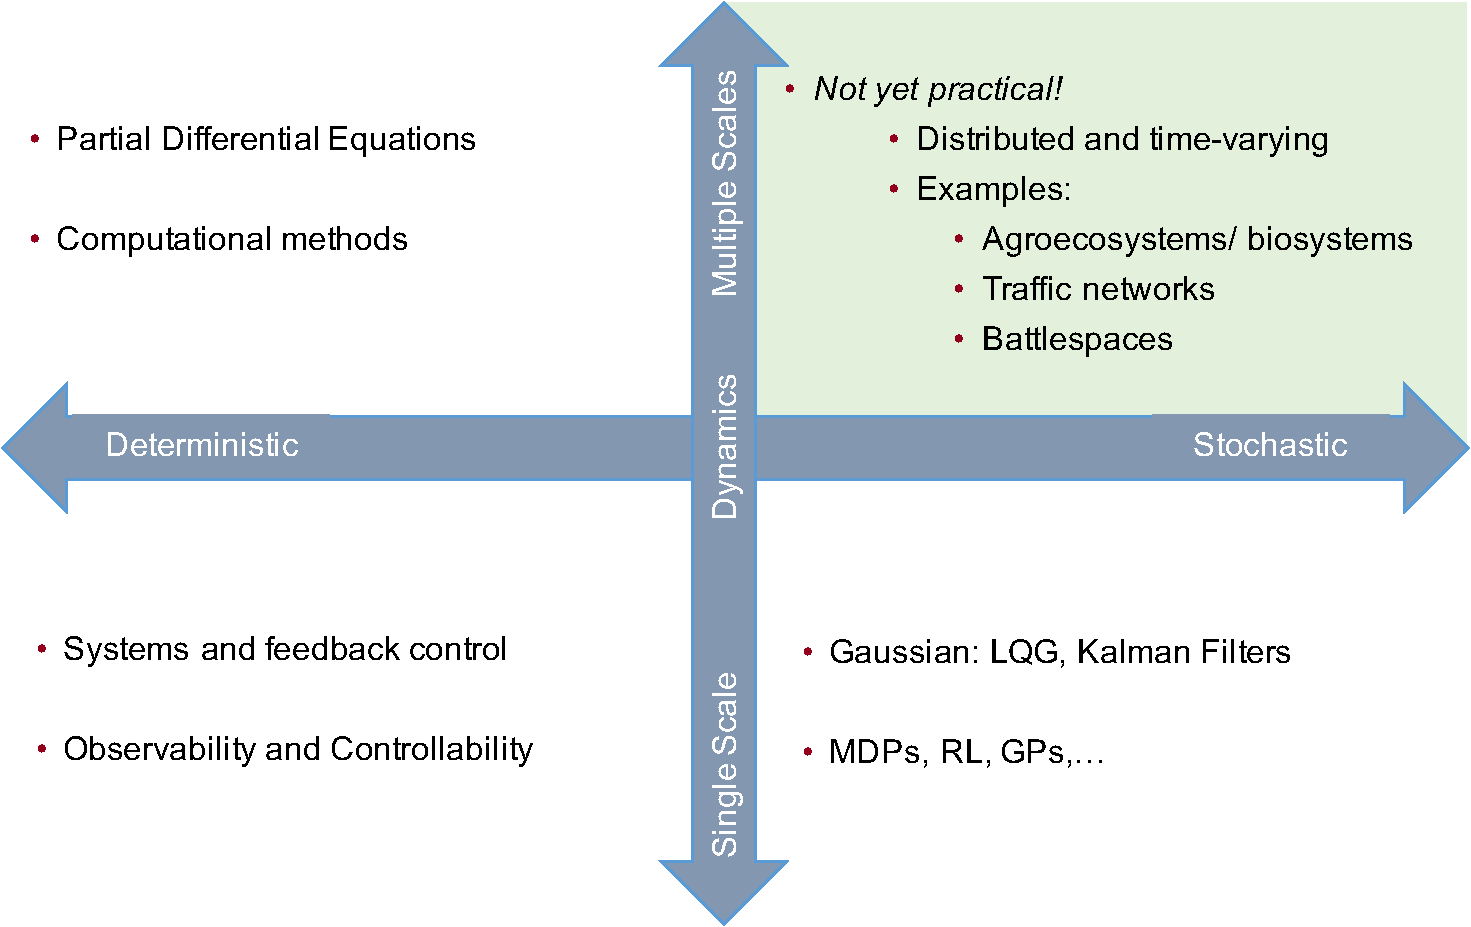
\includegraphics[width=\columnwidth]{Figure 2}
		\caption{Modeling, monitoring, and controlling dynamical systems with complex and uncertain dynamics, such as agricultural, traffic, or weather monitoring systems, presents exciting open challenge for the controls community. The bottom left quadrant describes linear and time-invariant systems with single-scale dynamics, for which the theory of feedback control of dynamical systems is often sufficient. The bottom right quadrant shows stochastic single-scaled systems, where approaches such as Kalman Filters and Gaussian optimization have marked several successes of control systems, enabling endeavors from lunar landings to GPS navigation. The top left quadrant denotes systems with dynamics at multiple scales, where the efficient computation of solutions to Partial Differential Equations (PDEs) is an highly active area of research. Fundamental theoretical advances and practical algorithms are needed, however, to enable autonomous decision making for distributed stochastic Cyber Physical Systems with dynamics at multiple scales – shown in the top right quadrant – such as distributed agricultural robotic systems, traffic networks, and weather monitoring systems with mobile and stationary sensors.}
	\label{fig:cps_soa}
\end{figure}


\subsection*{Outline of the article and relationship to prior work by the authors}
 We begin the rest of the article by summarizing some related work in machine learning in this area.  ``\nameref{sb:featspace}'' discusses the concept of feature spaces and its importance in machine learning in a broader context. We then formulate the problem, introduce \emph{Kernel Observers (KO)}, and develop the main theoretical and algorithmic results.
This is followed by some results on the expected number of randomly placed sensors required to monitor a spatiotemporal process in the context of our model. An extension to the KO method called \emph{Evolving Gaussian Processes (E-GP)} is presented that learns one model for multiple, similar spatiotemporal processes, the efficacy of which on real-world CFD data is presented in Sidebar \emph{Learning Fluid Flows with Evolving Gaussian Processes}.
Elements of the work presented in this paper first appeared in Neural Information Processing Systems (NIPS 2016) (\cite{Kingravi16_NIPS,whitman2016NIPSworkshop}), IEEE CDC 2015 conference \cite{Kingravi:2015a}, the Conference on Robot Learning (CoRL 2017) \cite{whitman2017learning} and IEEE ACC 2018 conference \cite{Maske18_ACC}.  This paper presents a comprehensive set of results and fills in the missing links in a single encompassing publication, and introduces new results on observability in the presence of random sensor placement, and connections to Koopman operator theory. As such, we have focused in this article mostly on the fundamental theory and practical algorithms for modeling, estimation, and control, while the details of how to optimally implement the presented algorithms are omitted. Instead, an open-source code-base is made available in MATLAB at \url{http://daslab.illinois.edu/software.html} or at \url{https://github.com/hkingravi/FunctionObservers} and in Python on GitHub at \url{https://github.com/hkingravi/funcobspy}.

